\documentclass[12pt,a4paper]{article}

\usepackage[utf8]{inputenc}
\usepackage[T1]{fontenc}
\usepackage[spanish]{babel}
\usepackage[margin=2.2cm]{geometry}
\usepackage{setspace}
\onehalfspacing
\usepackage[sfdefault]{carlito}
\usepackage{graphicx}
\usepackage{hyperref}
\usepackage{xcolor}
\usepackage{enumitem}

\hypersetup{colorlinks=true, linkcolor=blue, urlcolor=blue, citecolor=blue}

\newcommand{\Universidad}{Universidad Internacional de La Rioja (UNIR)}
\newcommand{\Asignatura}{Informática Gráfica y Visualización}

\title{\textbf{Laboratorio 1: Introducción a OpenGL}\\Reloj analógico estático}
\author{Sergio Andrés Majé Franco}
\date{\Asignatura \\ \Universidad \\ 18 de mayo de 2026}

\begin{document}

\maketitle
\tableofcontents
\newpage

\section{Introducción}
La práctica propone desarrollar un programa en C con OpenGL capaz de dibujar un reloj analógico estático. El objetivo principal del laboratorio es familiarizarse con las primitivas básicas de dibujo y con la representación geométrica de elementos sencillos en una escena bidimensional.

La solución implementada genera la esfera del reloj, las doce marcas horarias y las manillas de hora, minuto y segundo. Aunque el reloj no incorpora animación, sí toma la hora del sistema al iniciar la ejecución para producir una representación estática coherente.

\section{Descripción de la solución}
\subsection{Enfoque general}
La aplicación se ha construido con OpenGL clásico e integra un contexto gráfico sobre X11/GLX. Esta decisión se ha tomado para ajustarse al entorno disponible durante el desarrollo y mantener una implementación sencilla, centrada en el uso de primitivas de dibujo y transformaciones geométricas básicas.

El dibujo se realiza en coordenadas cartesianas 2D mediante una proyección ortográfica. De este modo, el reloj conserva su proporción al redimensionar la ventana y se evita la deformación de la circunferencia.

\subsection{Construcción geométrica del reloj}
La generación del reloj se basa en relaciones trigonométricas simples:

\begin{itemize}[leftmargin=*]
    \item la circunferencia exterior se aproxima mediante un conjunto de segmentos distribuidos uniformemente;
    \item las doce marcas horarias se calculan a partir de ángulos separados cada 30 grados;
    \item las manillas se construyen como segmentos con distinta longitud y grosor según representen horas, minutos o segundos;
    \item los ángulos de las manillas se obtienen a partir de la hora capturada al inicio del programa.
\end{itemize}

Este enfoque permite que la solución sea clara desde el punto de vista académico, ya que hace explícito cómo se pasa de un valor angular a sus coordenadas cartesianas dentro del plano.

La base geométrica del dibujo parte de situar el centro del reloj en el origen del sistema de coordenadas. A partir de ese punto, cualquier elemento del reloj puede describirse mediante un radio y un ángulo. Para convertir esa representación polar en coordenadas cartesianas se usan las expresiones habituales:

\begin{verbatim}
x = r * cos(theta)
y = r * sin(theta)
\end{verbatim}

Con esta idea se obtiene primero la circunferencia principal. En lugar de calcularla como una curva continua, se recorre el ángulo completo desde 0 hasta 360 grados con pequeños incrementos uniformes. Cada ángulo genera un punto de la forma $(r \cos \theta, r \sin \theta)$ y la unión secuencial de esos puntos construye una aproximación poligonal visualmente suave.

Las marcas horarias siguen el mismo principio, pero en este caso no se dibuja una curva, sino doce segmentos radiales. Cada marca se sitúa separada 30 grados de la siguiente, ya que una vuelta completa tiene 360 grados y el reloj se divide en 12 horas. Para cada marca se calculan dos puntos: uno interior y otro exterior. Ambos comparten el mismo ángulo, pero tienen radios distintos. Así se obtiene un segmento corto que apunta desde el interior de la esfera hacia el borde exterior.

El cálculo de las manillas utiliza un criterio análogo. Cada una se representa como un segmento que parte del origen y termina en un punto calculado a partir de su longitud y de su ángulo. La manilla de los segundos avanza 6 grados por segundo, porque 360/60 = 6. La manilla de los minutos también avanza 6 grados por unidad, incorporando además la fracción correspondiente de los segundos para mejorar la coherencia visual. La manilla de las horas avanza 30 grados por hora, ya que 360/12 = 30, y además incorpora la fracción de avance de los minutos para que no quede fijada exactamente sobre una marca salvo en horas cerradas.

Para adaptar el sentido matemático de los ángulos al comportamiento esperado en un reloj analógico, el ángulo de referencia se desplaza de forma que las 12 queden en la parte superior. En otras palabras, se toma como referencia inicial 90 grados y después se resta el desplazamiento angular correspondiente a cada manilla. Gracias a ello, el reloj queda orientado como un reloj convencional y no como una circunferencia trigonométrica estándar.

\section{Implementación}
\subsection{Estructura principal}
La implementación queda concentrada en el archivo \texttt{solution.c}, que contiene la inicialización de la ventana, la captura de la hora, la configuración de la proyección 2D y las funciones auxiliares para dibujar los distintos elementos del reloj.

La lógica principal se organiza alrededor de tres responsabilidades:

\begin{itemize}[leftmargin=*]
    \item crear el contexto gráfico y la ventana de renderizado;
    \item calcular la geometría necesaria para la esfera, las marcas y las manillas;
    \item renderizar el resultado final y mantenerlo estático durante la ejecución.
\end{itemize}

\subsection{Decisiones relevantes}
Durante la implementación se han adoptado varias decisiones orientadas a mejorar la claridad del resultado:

\begin{itemize}[leftmargin=*]
    \item se captura la hora una sola vez porque el enunciado exige un reloj estático;
    \item se usan colores y grosores distintos para diferenciar visualmente las manillas;
    \item se reconfigura la proyección cuando la ventana cambia de tamaño para conservar la relación de aspecto;
    \item se añade un punto central para cerrar visualmente la unión de las manillas.
\end{itemize}

\section{Resultado}
\subsection{Captura del programa}
\IfFileExists{../captures/reloj.png}{%
    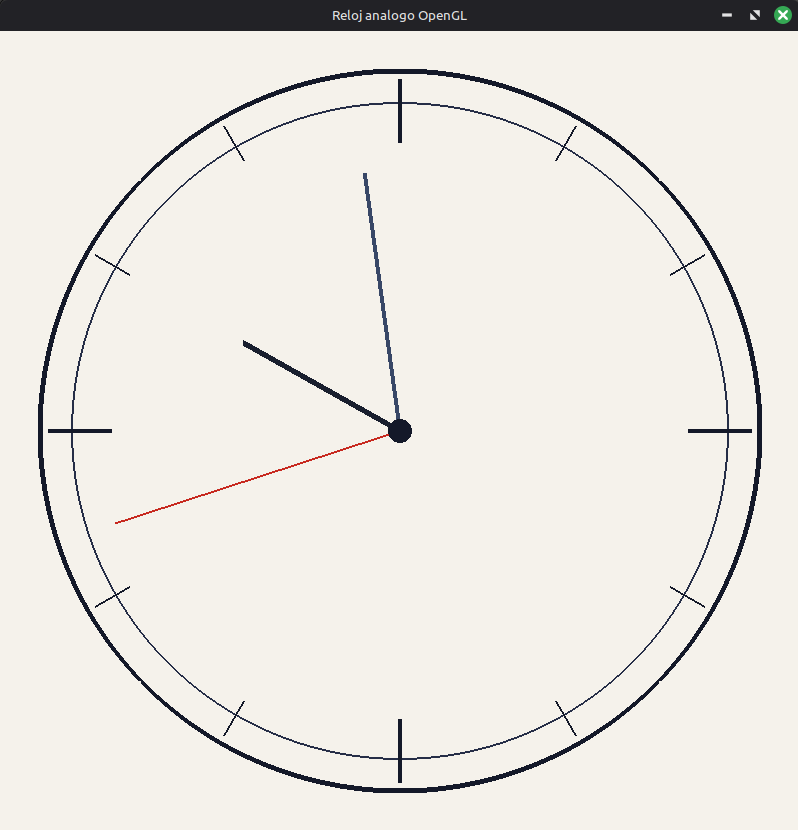
\includegraphics[width=0.72\textwidth]{../captures/reloj.png}
}{%
    \fcolorbox{black}{gray!10}{%
        \parbox{0.72\textwidth}{%
            Captura pendiente de incorporar en \texttt{captures/reloj.png}.
        }%
    }%
}

\smallskip

\textbf{Figura 1.} Ejecución del reloj analógico implementado.

\subsection{Funcionamiento}
\textbf{¿Funciona bien tu programa?}

Sí. El programa está diseñado para mostrar correctamente un reloj analógico estático con una distribución regular de las doce marcas horarias y con las manillas orientadas de acuerdo con la hora obtenida al inicio de la ejecución. Además, el dibujo mantiene una proporción visual adecuada al redimensionar la ventana.

\section{Limitaciones y fallos detectados}
\textbf{¿Qué fallos existen?}

La solución funciona correctamente dentro del alcance de la práctica, pero presenta varias limitaciones que conviene dejar documentadas:

\begin{itemize}[leftmargin=*]
    \item depende de un entorno gráfico compatible con OpenGL y X11/GLX, por lo que no puede ejecutarse en entornos sin servidor gráfico accesible;
    \item la hora no se actualiza durante la ejecución, ya que se toma una única muestra al inicio para respetar el requisito de reloj estático;
    \item la circunferencia está aproximada por segmentos, por lo que su suavidad visual depende del número de divisiones utilizado;
    \item la implementación está orientada al entorno Linux disponible durante el desarrollo, aunque el laboratorio original menciona también el uso de GLUT en otros sistemas.
\end{itemize}

\section{Conclusiones}
La práctica cumple el objetivo de introducir el uso de OpenGL para dibujar primitivas simples y componer con ellas una figura reconocible. Desde el punto de vista didáctico, el reloj analógico resulta adecuado porque obliga a combinar geometría elemental, coordenadas en el plano, control de proporciones y una organización mínima del flujo de renderizado.

Además, la solución deja una base reutilizable para ejercicios posteriores, ya que separa con claridad la creación de la ventana, la configuración de la proyección y el cálculo geométrico de los elementos dibujados.

Finalmente, el informe se encuentra en el siguiente repositorio:

\href{https://github.com/smaje99/computer-graphics-and-visualization-unir}{https://github.com/smaje99/computer-graphics-and-visualization-unir}

Además, junto a este documento se adjunta un archivo comprimido que también incluye el informe y el resto del material desarrollado para la práctica.

\end{document}
